% Diapo d'intro
% \begin{frame}[c]
%   \frametitle{Context}
% %rajouter le titre (version courte) dans toute les slides
% \begin{center}
%   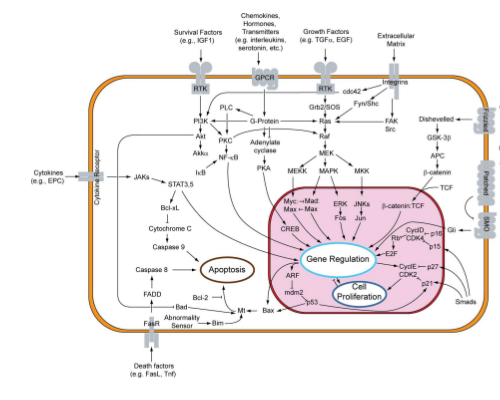
\includegraphics[scale=0.55]{images/cellule_description_lui.png}
% \end{center}
% \begin{center}
% {\tiny \color{darkgreen}[\citelui]}
% \end{center}
% 
% %\tcite{Wikipédia}
% 
% \begin{itemize}
% \item Cellular processes are driven by networks of biological interactions.
% \item Formal modelling and analysis of Biological Regulatory Network.
% \item Static analysis of properties.
% \end{itemize}
% 
% %Cellular processes are driven by networks of biological reactions. Cells rely on the tight coordination of these pathways to achieve proper functioning.
% %With the help of signaling pathway, a cell senses changes in its environnement or internal state. This information is then passed on via cascades of biochemical 
% %reactions to the appropriate mechanisms which respond by modifying the metabolic and transcriptiona activities. this in turn modifies the behavior of the cell.
% 
% %Consequently, the dynamics of biopathways play a crucial role in determinig cellular functions.
% 
% %Examples: circadian rhythm, the apoptosis pathway inducing programmed cell death, cell differentiation.
% 
% %\textcolor{couleurtheme}{$\Rightarrow$} \fbox{\tval{\large The need of comprehension of biological systems}} \textcolor{couleurtheme}{$\Leftarrow$}
% 
% 
% %\textcolor{couleurtheme}{$\Rightarrow$} \fbox{\tval{\large Allow efficient translation from Process Hitting to BRN}} \textcolor{couleurtheme}{$\Leftarrow$}
% 
% \end{frame}

\begin{frame}[c]
  \frametitle{Introduction à la notion de bifurcation}
 \framesubtitle{Différenciation des cellules souches}

\begin{center}
  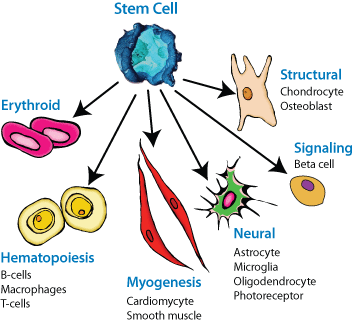
\includegraphics[scale=0.42]{images/illustration_differentiation.png}
  % \multiinclude[format=gif, scale=0.5]{images/illustration_differentiation.gif}
\end{center}
\begin{center}
{\tiny \color{darkgreen} [https://www.systembio.com/stem-cell-research/differentiation-reporters/overview]}
\end{center}
%\tcite{system Biosciences}

\begin{itemize}
\item \tval{Différenciation} $\Longrightarrow$ Perte de capacité %expliquer la notion de perte de capacité sur la figure.
\item Quelles transitions (opérations) sont responsables des \tval{bifurcations} ? 
\item \`A partir de quels états ?
\end{itemize}
\end{frame}

\begin{frame}[c]
  \frametitle{Approximation des bifurcations}
%system dynamique
%Bifurcations
%rajouter une autre image pour illustrer pour qu'on voit que c'est toujours des états qui changes
% \begin{center}
%   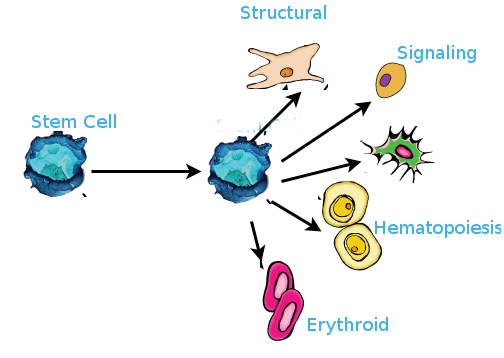
\includegraphics[scale=0.3]{images/illustration_differentiation_newio1.png}
%   % \multiinclude[format=gif, scale=0.5]{images/illustration_differentiation.gif}
% \end{center}
\begin{center}
\begin{tikzpicture}
 \node[esdef] (bif ) at (0,1) {\begin{tabular}{c} Bifurcations \\ \textcolor{red}{PSPACE Complet} \end{tabular}};
 
 \node[esdef] (bifctl) at (0,-2) {\begin{tabular}{c}$EF \ g_1  \wedge \cdots$  \\ (CTL) \end{tabular}};
 
 \node[esdef] (pl) at (6,-2) {\begin{tabular}{c}Programme logique \\ (SAT/ASP) \end{tabular}};
 
 \node[esdef] (abif) at (6,1) {\begin{tabular}{c}Approximation \\ des bifurcations \end{tabular}};
                                                                                  
 
  
 \draw[->] (bif) -- (bifctl);
 \draw[->] (bifctl)-- node[below=5pt,midway]{\textcolor{black}{\textbf{Approximation}}}node[above=5pt,midway]{\textcolor{black}{\textbf{IA + PL}}} (pl);
 \draw[->] (pl) -- (abif);
 
\end{tikzpicture}
\end{center}


\begin{liste}
%\item Les transitions de bifurcation peuvent être exprimées dans la logique temporelle
%\item {\bf "Approximation"} :\\ vérification d'une formule CTL (\tval{PSPACE (complet)})\\
%       $\Rightarrow$ Problème NP qui peut être aisément exprimé en SAT/ASP %trouver l'orthagraphe de easely
\item {\bf Contribution} : $$
\left\{
    \begin{array}{lcl}
        \mbox{PL (Programmation logique)} &\\  %rajouter un signe entre les deux
        \mbox{+} & \Longrightarrow \mbox{\tval{approximations formelles des bifurcations}} \\
        \mbox{IA (Interprétation abstraite)} &
    \end{array}
\right.
$$ 
\end{liste}
\end{frame}
